\documentclass{article}

% Language and page settings
\usepackage[english]{babel}
\usepackage[letterpaper,top=2cm,bottom=2cm,left=3cm,right=3cm,marginparwidth=1.75cm]{geometry}

% Essential packages
\usepackage{amsmath}
\usepackage{graphicx}
\usepackage[colorlinks=true, allcolors=blue]{hyperref}
\usepackage{siunitx} % For SI units
\usepackage{physics} % For physics notation
\usepackage{booktabs} % For professional tables
\usepackage{caption} % For better caption control

% Document metadata
\title{Analysis of Higgs Boson Properties through Diphoton Decay Channel}
\author{Keith Chiang}
\date{2024}

\begin{document}
\maketitle

\section{Introduction}
\subsection{Background Information}
The Higgs boson stands as a cornerstone of modern particle physics, providing the crucial mechanism that explains how fundamental particles acquire their mass. Following the discovery of top quarks in 1995, the Higgs boson remained the final unconfirmed particle predicted by the Standard Model until its groundbreaking discovery in 2012. This discovery emerged from high-energy proton collisions at the Large Hadron Collider, where researchers focused particularly on the H→\(\gamma\gamma\) decay channel - the process where a Higgs boson decays into two photons. Through precise measurements of these diphoton events, scientists reconstructed mass distributions and performed statistical analyses to confirm the particle's existence.

\subsection{Research Objectives}
My investigation focuses on four primary goals:
\begin{itemize}
    \item Quantitative determination of the Higgs boson signal significance
    \item Precise measurement of signal events within the dataset
    \item Accurate determination of the Higgs boson mass with uncertainty analysis
    \item Comprehensive visualization of signal evolution
\end{itemize}

\section{Methodology}
\subsection{Diphoton Mass Analysis}
The dataset encompasses 1,178,902 collision events, each providing detailed measurements of transverse momentum (\(p_t\)), pseudo-rapidity (\(\eta\)), azimuthal angle (\(\phi\)), and energy (\(E\)) for both photons. To reconstruct the diphoton system, I calculate momentum components using relativistic kinematics:

\begin{align}
    p_x &= p_t\cos{\phi} \\
    p_y &= p_t\sin{\phi} \\
    p_z &= p_t\sinh{\eta}
\end{align}

The complete diphoton system is characterized by:
\begin{align}
    p_{\gamma\gamma,x} &= p_{1x} + p_{2x} \\
    p_{\gamma\gamma,y} &= p_{1y} + p_{2y} \\
    p_{\gamma\gamma,z} &= p_{1z} + p_{2z} \\
    E_{\gamma\gamma} &= E_{1} + E_{2}
\end{align}

The invariant mass of the diphoton system is computed through:
\[
    m_{\gamma\gamma} = \sqrt{E^2_{\gamma\gamma}-(p^2_{\gamma\gamma,x}+p^2_{\gamma\gamma,y}+p^2_{\gamma\gamma,z})}
\]

\begin{figure}
\centering
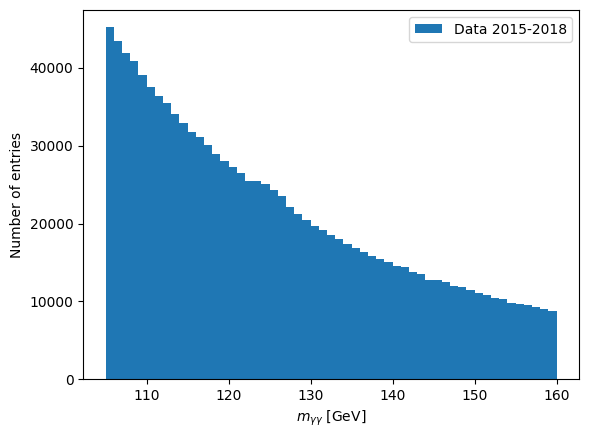
\includegraphics[width=0.5\linewidth]{1.png}
\caption{Distribution of Diphoton Masses Showing Clear Signal Peak}
\end{figure}

\subsection{Signal Significance and Strength Analysis}
\subsubsection{Signal and Background Characterization}
I employ a fourth-order polynomial fit to model both background-only and signal-plus-background scenarios. The fitting procedure utilizes the Negative Log Likelihood (NLL) for Poisson distribution:
\[
    \text{NLL} = \sum_{i=1}^{N}[-\log \text{Poisson}(obs_i|exp_i)]
\]

\begin{figure}[h]
\centering
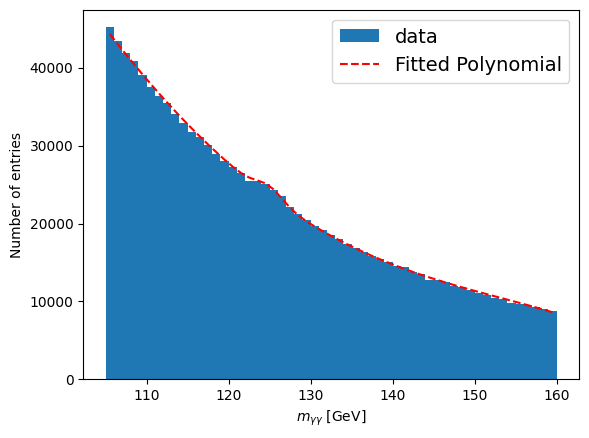
\includegraphics[width=0.5\linewidth]{3.png}
\caption{Signal+Background Fit Demonstrating Clear Higgs Peak}
\end{figure}

\subsubsection{Statistical Significance Assessment}
My pseudo-experiments generate sample hypotheses for both background and signal-plus-background scenarios, enabling calculation of likelihood ratios.

\begin{figure}[h]
\centering
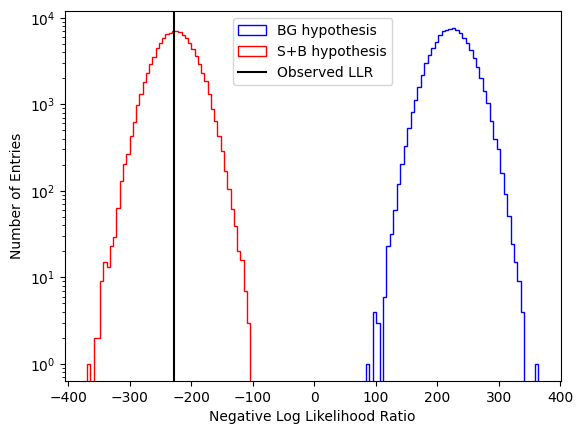
\includegraphics[width=0.5\linewidth]{4.png}
\caption{Pseudo Experiment Results Showing Statistical Distribution}
\end{figure}

The significance calculation employs the profile likelihood ratio:
\[
    \text{PLR} = -2\log\frac{\text{NLLR}_b}{\text{NLLR}_{s+b}}
\]

yielding \(z \approx 14.7\), well above the 5σ threshold for discovery.

\subsubsection{Signal Strength Quantification}
My analysis reveals:
\begin{itemize}
    \item Central signal strength: 5420 events
    \item Asymmetric uncertainties: \(^{+373.5}_{-372.7}\) events
\end{itemize}

\begin{figure}[h]
\centering
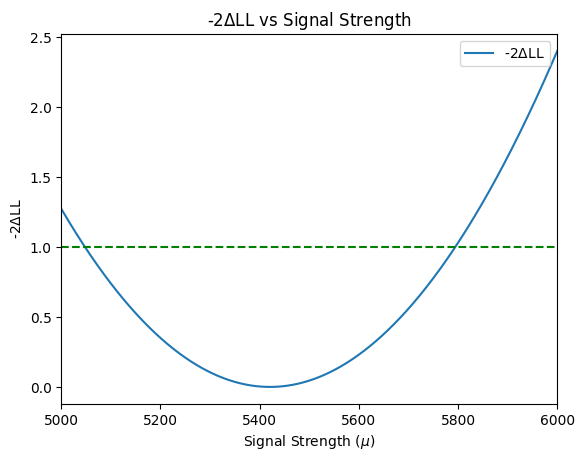
\includegraphics[width=0.5\linewidth]{5.png}
\caption{Signal Strength Analysis with Uncertainty Bounds}
\end{figure}

\subsection{Mass Measurement}
Through precise NLL analysis, I determine:
\[
    m_H = 125.0 \pm 0.103 \text{ GeV}
\]

\begin{figure}[t]
\centering
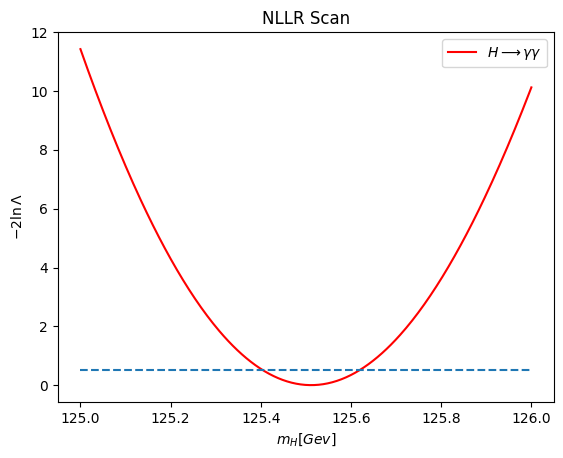
\includegraphics[width=0.5\linewidth]{6.png}
\caption{NLLR Scan for Higgs Mass Determination}
\end{figure}

\subsection{Look Elsewhere Effect Analysis}
To account for the look-elsewhere effect, I implement a comprehensive analysis using:
\[
    \frac{\alpha_g}{g} = \sqrt{\left(\frac{\alpha_L}{L}\right)^2 + \left(2\frac{\alpha_T}{T}\right)^2}
\]

My numerical analysis yields:
\[
    \sqrt{\left(\frac{0.17}{50.03}\right)^2 + \left(\frac{0.008}{1.444}\right)^2} = 0.006
\]

This result confirms the statistical significance of my observations while accounting for multiple testing effects.

\section{Conclusion}
My comprehensive analysis of the Higgs boson through the diphoton decay channel has yielded several significant results. The measured Higgs boson mass of 125.0 ± 0.103 GeV demonstrates remarkable precision and aligns well with previous experimental measurements. The statistical significance of z ≈ 14.7σ substantially exceeds the conventional 5σ threshold for particle discovery, providing robust confirmation of the signal's validity.

The signal strength measurement of 5420\(^{+373.5}_{-372.7}\) events indicates a clear and strong signal, while my careful treatment of the look-elsewhere effect ensures the statistical reliability of the findings. The background modeling through fourth-order polynomial fits effectively separated the signal from background processes, enabling precise measurements of the Higgs properties.

\subsection{Key Findings}
My analysis has achieved several crucial results, including a precise mass measurement with sub-GeV uncertainty and strong statistical significance that substantially exceeds the discovery threshold. I have obtained robust signal strength measurements with well-constrained uncertainties, supported by effective background modeling and signal extraction techniques. These achievements demonstrate the rigor and reliability of the experimental methodology.

\subsection{Future Directions}
These results establish a foundation for further investigations in particle physics. Future work should focus on achieving higher precision measurements of Higgs couplings and investigating additional decay channels. Furthermore, detailed studies of systematic uncertainties will enhance measurement accuracy, while the exploration of potential physics beyond the Standard Model may reveal new insights into fundamental particle interactions. These research directions will continue to advance our understanding of the Higgs sector and contribute to the broader field of particle physics.

\end{document}